\begin{example}[Nested Loop with Related Iterators]
  \label{ex:threeNestedWhile}
  %
  %
  { \small
\begin{figure}
\centering
\begin{subfigure}{.4\textwidth}
  \begin{centering}
  {\footnotesize
  $
  \begin{array}{l}
      \kw{relatedNestedWhile}(n, m, N) \triangleq \\
      \clabel{ \assign{i}{0} }^{0} ; \\
          \ewhile ~ \clabel{i < n}^{1} ~ \edo ~ \\
          \qquad \Big(
           \clabel{\assign{j}{m}}^{2} ;\\
           \qquad \ewhile ~ \clabel{j > 0}^{3} ~ \edo ~ \\
           \qquad \qquad \Big(
            \clabel{\assign{j}{j-1}}^{4};
            \clabel{\assign{w}{i}}^{5};\\
            \qquad \qquad \ewhile ~ \clabel{w < N}^{6} ~ \edo ~
            \Big(
              \clabel{\assign{w}{w + 1}}^{7}
                \Big); \\
                \qquad \qquad \clabel{\assign{i}{w}}^{8}
                \Big); \\
                \qquad \clabel{\assign{i}{i+1}}^{9}
            \Big)
      \end{array}
  $
  }
  \caption{}
  \end{centering}
  \end{subfigure}
\begin{subfigure}{.5\textwidth}
  \begin{centering}
%   \todo{abstract-cfg for two round}
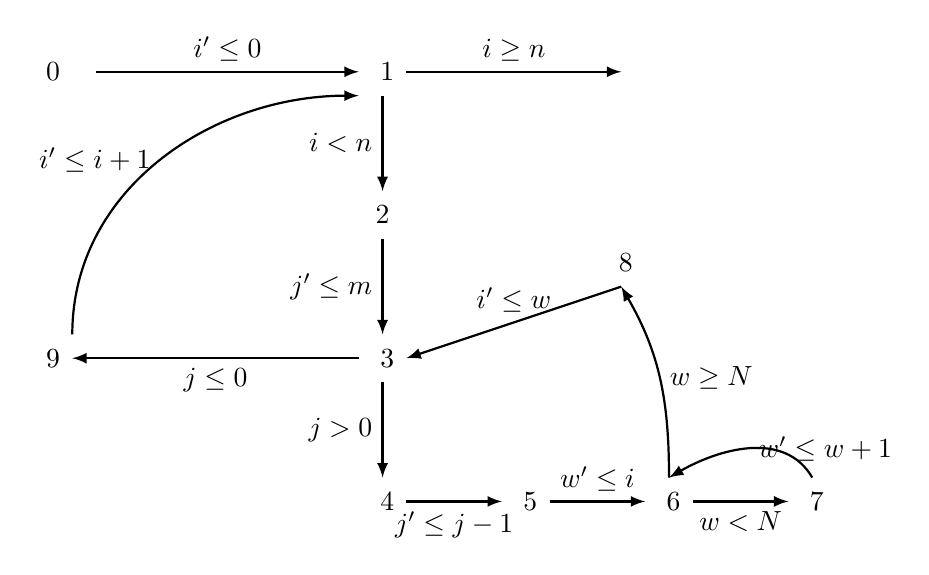
\begin{tikzpicture}[scale=\textwidth/20cm,samples=200]
\draw[] (-7, 10) circle (0pt) node{{ $0$}};
\draw[] (0, 10) circle (0pt) node{{ $1$}};
\draw[] (6, 10) circle (0pt) node {{$\lex$}};
\draw[] (0, 7) circle (0pt) node{{$2$}};
\draw[] (0, 4) circle (0pt) node{{ $3$}};
\draw[] (-7, 4) circle (0pt) node{{ $9$}};
\draw[] (0, 1) circle (0pt) node{{ $4$}};
\draw[] (3, 1) circle (0pt) node{{ $5$}};
\draw[] (6, 1) circle (0pt) node{{ $6$}};
\draw[] (9, 1) circle (0pt) node{{ $7$}};
\draw[] (5, 6) circle (0pt) node{{ $8$}};
% Counter Variables
%
% Control Flow Edges:
\draw[ thick, -latex] (-6, 10)  -- node [above] {$i' \leq 0$}(-0.5, 10);
\draw[ thick, -latex] (0, 9.5)  -- node [left] {$i < n$} (0, 7.5) ;
\draw[ thick, -latex] (0, 6.5)  -- node [left] {$j' \leq m$} (0, 4.5) ;
\draw[ thick, -latex] (0, 3.5)  -- node [left] {$j > 0$} (0, 1.5) ;
\draw[ thick, -latex] (-0.5, 4)  -- node [below] {$j \leq 0$} (-6.5, 4) ;
\draw[ thick, -latex] (-6.5, 4.5)  to  [out=90,in=180]  node [left] {$i' \leq i + 1$ }(-0.5, 9.5);
\draw[ thick, -latex] (0.5, 10)  -- node [above] {$i \geq n$}  (5, 10);
\draw[ thick, -latex] (0.5, 1)  -- node [below] {$j' \leq j - 1$}  (2.5, 1);
\draw[ thick, -latex] (3.5, 1)  -- node [above] {$w' \leq i$}  (5.5, 1);
\draw[ thick, -latex] (6.5, 1)  -- node [below] {$w < N$}  (8.5, 1);
\draw[ thick, -latex] (6, 1.5)  to [out=90,in=-60] node [right] {$w \geq N$}  (5, 5.5);
\draw[ thick, -latex] (9, 1.5)  to  [out=120,in=30] node [right] {$w' \leq w + 1$}  (6, 1.5);
\draw[ thick, -latex] (5, 5.5)  to  node [above] {$i' \leq w$ }(0.5, 4);
\end{tikzpicture}
\caption{}
  \end{centering}
  \end{subfigure}
\caption{
(a) The Example of Nested Loop with Related Iterators
  (b) The Abstract Execution Control Flow Graph}
    \label{fig:threeNestedWhile}
\end{figure}
}
\end{example}

\begin{enumerate}
  \item  \textbf{The Abstract Control Flow Graph} is generated in Figure~\ref{fig:threeNestedWhile}(b).

  \item \textbf{Program Refinement}
  \\
  The \textbf{simple transition paths} are
  %  are computed as follows,
  \\
$
      \begin{array}{llll}
          \tpath_0 = (0 \to 1)
          &
          \tpath_1 = (1 \to 2 \to 3)
          &           
          \tpath_2 = (3 \to 4 \to 5 \to 6)
          &
          \tpath_3 = (6 \to 7 \to 6)
          \\
          \tpath_6 = (1 \to \lex)
          &
          \tpath_4 = (6 \to 8 \to 3)
          &
          \tpath_5 = (3 \to 9 \to 1)
      \end{array}
$
  \\
  The \textbf{repeat patterns}
  for the loop that its header is
  \\
  % the repeat pattern for the loop that its header is at the program point 
  % loop with header 
  at the program point 
  $1$ is $\rprepeat(\tpath_1; \tpath_5)$; \\
  % loop with header 
  at the program point $3$ is $\rprepeat(\tpath_2; \tpath_4)$;
  \\
  at the program point $6$ is $\rprepeat(\tpath_3)$.
  \\
  The \textbf{refined program
  % \footnote{$\rprog$ is used as the inputs (/ arguments) of the computations in the following steps.
  % For concise, it is omitted since all the arguments in the following computations are referring to the same $\rprog$.}
  } is
\\
  $
  \rprog = \tpath_0 ; 
  \rpchoose{1: \rprepeat(\tpath_1; \rpchoose{3: \rprepeat(\tpath_2; \rpchoose{6 : \rprepeat(\tpath_3)}; \tpath_4)}; \tpath_5)}; \tpath_6
$
  % \highlight{$\rprog$ is used as the inputs (/ arguments) of the computations in the following steps.
  % For concise, it is omitted since all the arguments in the following computations are referring to the same $\rprog$.}
  \item \textbf{Ranking Function Computation}:
  \\
    The \textbf{ranking function / (local bound)}  assigned to each edge is as follows,
      \\  
      $\locbound(0 \to 1) = 1$ 
      \quad $\locbound(1 \to \lex) = 1$
      \quad $\locbound(1 \to 2) = i$
      \quad $\locbound(2 \to 3) = i$ 
      \quad $\locbound(3 \to 9) = i$ 
      \quad $\locbound(9 \to 1) = i$ 
      \quad $\locbound(3 \to 4) = j$
      \quad $\locbound(4 \to 5) = j$ 
      \quad $\locbound(5 \to 6) = j$ 
      \quad $\locbound(6 \to 8) = j$ 
      \quad $\locbound(8 \to 3) = j$ 
      %%%
      \quad $\locbound(6 \to 7) = w - n + N$ 
      \quad $\locbound(7 \to 6) = w - n + N$ 
  \\
  The bound on the maximum value of each ranking function, i.e., the \textbf{ranking function bound} is as follows,
  \\
  $\varinvar(i) = n$  \quad
  $\varinvar(j) = m * n$  \quad
  $\varinvar(w) = n$  \quad
  $\varinvar(w - n + N) = N$ 
  \\
  The \textbf{path-insensitive transition bound} for each edge:
  \\
  $\absclr(0 \to 1) = 1$ 
  \quad $\absclr(1 \to \lex) = 1$
  \quad $\absclr(1 \to 2) = n$
  \quad $\absclr(2 \to 3) = n$ 
  \quad $\absclr(3 \to 9) = n$ 
  \\
  \quad $\absclr(9 \to 1) = n$ 
  \quad $\absclr(3 \to 4) = m * n$
  \quad $\absclr(4 \to 5) = m * n$ 
  \quad $\absclr(5 \to 6) = m * n$ 
  \\
  \quad $\absclr(6 \to 8) = m * n$ 
  \quad $\absclr(8 \to 3) = m * n$ 
  %%%
  \quad $\absclr(6 \to 7) = N$ 
  \quad $\absclr(7 \to 6) = N$ 
  % ? following steps. 
  \item \textbf{Outside-In Algorithm}:\\
  The \textbf{Outside-In} bound for every $\rpattern$ w.r.t. the refined program $\rprog$ is as follows,
  %  and every nested repeat patterns.
  \\
$\outinB(\tpath_0) = 1$
\quad
$\outinB(\tpath_6) = 1$
\quad
$\outinB(6 : \rprepeat(\tpath_3)) = N $
\\
$\outinB(3: \rprepeat(\tpath_2; 6 : \rprepeat(\tpath_3); \tpath_4)) = m $
\\
$\outinB(1: \rprepeat(\tpath_1; 3: \rprepeat(\tpath_2; 6 : \rprepeat(\tpath_3); \tpath_4); \tpath_5)) = n - N $
\item \textbf{Inside-Out Algorithm}:
\begin{itemize}
  \item \textbf{Repeat Chain Set}
  \\
  $\rpchset(1, \tpath_1) = 
  \{1: \rprepeat(\tpath_1; 3: \rprepeat(\tpath_2; 6 : \rprepeat(\tpath_3); \tpath_4); \tpath_5) \to \tpath_1\}$
  \\
  $\rpchset(1, \tpath_5) = \{1: \rprepeat(\tpath_1; 3: \rprepeat(\tpath_2; 6 : \rprepeat(\tpath_3); \tpath_4); \tpath_5) \to \tpath_5\}$
  \\
  $\rpchset(3, \tpath_2) = \{3: \rprepeat(\tpath_2; 6 : \rprepeat(\tpath_3); \tpath_4) \to \tpath_2\}$
  \\
  $\rpchset(3, \tpath_4) = \{3: \rprepeat(\tpath_2; 6 : \rprepeat(\tpath_3); \tpath_4) \to \tpath_3\}$
  \\
  $\rpchset(6, \tpath_3) = \{6: \rprepeat(\tpath_3) \to \tpath_3\}$
  \\
  $\rpchset(\_, \_) = \emptyset$ 
  % \\
  \item \textbf{Repeat Chain Bound}
  % for every simple transition path $\tpath$ through its \emph{Repeat Chain}s
  \\
  $\rpchB(1, \tpath_1) = n - N$ \quad
  $\rpchB(1, \tpath_5) = n - N$ \quad
  $\rpchB(3, \tpath_2) = m$ \\
  $\rpchB(3, \tpath_4) = m$ \quad
  $\rpchB(6, \tpath_3) = N$ \quad \quad 
  $\rpchB(\_, \_) = \bot $ 
  %
  \item \textbf{Loop Chain}
  \\
  $\lpch(\tpath_1) = 1\to \tpath_1$ \quad
  $\lpch(\tpath_5) = 1\to \tpath_5$ \quad
  $\lpch(\tpath_2) = 1 \to 3 \to \tpath_2$ \quad
  $\lpch(\tpath_4) = 1 \to 3 \to \tpath_4$ \quad
  \highlight
  {$\lpch(\tpath_3) = 1 \to 3 \to 5 \to \tpath_3$ }\\
  $\lpch(\tpath_0) = \tpath_0$ \quad
  $\lpch(\tpath_6) = \tpath_6$ 
  \item \textbf{{Relative Loop Bound}}
  %  for every simple transition path $\tpath$ through its \emph{Loop Chain}
  \\
  $\rpchB(1, \tpath_1) = n - N$ \quad
  $\rpchB(1, \tpath_5) = n - N$ \quad
  $\rpchB(1, \tpath_2) = n$ \quad $\rpchB(3, \tpath_2) = m$ \quad
  $\rpchB(1, \tpath_4) = n$ \quad $\rpchB(3, \tpath_4) = m$ \quad
  \highlight{$\rpchB(1, \tpath_3) = 1$ \quad $\rpchB(3, \tpath_3) = 1$ \quad $\rpchB(5, \tpath_3) = N$} \quad
  $\rpchB(\_, \_) = \bot $ 
  \item \textbf{Inside-Out Bound}
  %  for every simple transition path $\tpath$
  \\
  $\inoutB(\tpath_1) = n - N$ \quad
  $\inoutB(\tpath_2) = n \times m$ \quad
  $\inoutB(\tpath_0) = 1$ 
  \\
  $\inoutB(\tpath_5) = n - N$ \quad
  $\inoutB(\tpath_4) = n \times m$ \quad
  $\inoutB(\tpath_6) = 1$ 
  \\
  $\inoutB(\tpath_3) = N$ \quad
  %   \item \textbf{Path-Sensitive Reachability-Bound} for every simple transition path $\tpath$
  % \\
  % $\inoutB(\tpath_1) = n - N$ \quad
  % $\inoutB(\tpath_2) = n \times m$ \quad
  % $\inoutB(\tpath_0) = 1$ 
  % \\
  % $\inoutB(\tpath_5) = n - N$ \quad
  % $\inoutB(\tpath_4) = n \times m$ \quad
  % $\inoutB(\tpath_6) = 1$ 
  % \\
  % $\inoutB(\tpath_3) = N$ \quad
\end{itemize}
\item \textbf{Path-sensitive Reachability-Bound}
%  on every program control location
\\
$\psRB(0) = \psRB(\lex) = 1$ \quad
$\psRB(1) = n - N + 1$ \quad
$\psRB(2) = \psRB(9) = n - N$ \quad
$\psRB(7) = N$
\\
$\psRB(3) = n - N + n \times m$ \quad
$\psRB(4) = \psRB(5) = \psRB(8) = n \times m$ \quad
$\psRB(6) = N + n \times m$ 
\\
For simplicity, the notation $\psRB(L)$ denotes every program point in this set $L$ has the same reachability-bound $\psRB(L)$.
Below is this compact notation w.r.t a set of program points, and we use the compact notation in the following examples.
\\
$\psRB(\{0, \lex\}) = 1$ \quad
$\psRB(\{1\}) = n - N + 1$ \quad
$\psRB(\{2, 9\}) = n - N$ \quad
$\psRB(\{3\}) = n - N + n \times m$ \quad
$\psRB(\{4, 5, 8\}) = n \times m$ \quad
$\psRB(\{7\}) = N$ \quad
$\psRB(\{6\}) = N + n \times m$ 
\end{enumerate}